\documentclass[12pt, t]{beamer}

\usepackage{graphicx}
\usepackage{amsmath}
\usepackage{setspace}
\usepackage{float} 
\usepackage{multido}
\usepackage{multirow}
\usepackage{array}
\usepackage{enumerate}
\usepackage{booktabs}
\usepackage{indentfirst} 
\usepackage[style=mla]{biblatex}
\usepackage{subcaption}
\usepackage{hyperref}
\usepackage{textpos}

\makeatletter
\let\@@magyar@captionfix\relax
\makeatother

\definecolor{Turquoise3}{RGB}{0, 134, 139}
\renewcommand{\emph}[1]{{\color{Turquoise3}\textsl{#1}}}
\newcommand{\C}{\mathbb{C}} \newcommand{\F}{\mathbb{F}} \newcommand{\R}{\mathbb{R}} \newcommand{\Q}{\mathbb{Q}}
\newcommand{\N}{\mathbb{N}}
\newcommand{\myseries}[2]{$#1_1,#1_2,\dots,#1_#2$}
\newcommand{\nullspace}{~\\[15pt]}
\newcommand{\remark}{\textbf{Remark: }}
\newcommand{\scp}[2]{\langle\,#1\,,\,#2\,\rangle} \newcommand{\scpp}{\langle\,\cdot\,,\,\cdot\,\rangle}


\usetheme{Madrid}
\setbeamertemplate{navigation symbols}{}

\addtobeamertemplate{frametitle}{}{
\begin{textblock*}{100mm}(0.85\textwidth,-1cm)

\includegraphics[height=1cm]{logo.png}
\end{textblock*}}

\definecolor{themecolor}{RGB}{25,25,112} 

\usecolortheme[named=themecolor]{structure}

\setbeamertemplate{items}[default]

\hypersetup{
    colorlinks=true,
    linkcolor=themecolor,
    filecolor=themecolor,      
    urlcolor=themecolor,
    citecolor=themecolor,
}

\title{VV285 RC Part II}
\subtitle{\textbf{Elements of Linear Algebra}\\``Matrices are just linear maps!"}
\institute[UM-SJTU JI]{Univerity of Michigan-Shanghai Jiao Tong University Joint Institute}
\author{Xingjian Zhang}

\begin{document}

\begin{frame}
    \titlepage
    \begin{center}
        
\includegraphics[height=2cm]{logo2.png}
    \end{center}
\end{frame}

\begin{frame}
    \frametitle{Something you need to pay attention to...}
    Think More and Be Interactive!
    \begin{itemize}
        \item Do think more about the question in ``()''. \\e.g. ``(How to prove?)''
        \item You are welcome to ask questions in a adequate manner.
        \item Please open your camera so that I can receive more feedbacks from you. (Makes our life easier!)
        \item The class is designed to be interactive. However, if you really do not want to be asked at all, please type an ``\_'' before your zoom name.
    \end{itemize}
\end{frame}

\section{Homework}
\begin{frame}
    \frametitle{Homework}
    Ability to use \textit{Mathematica} will help you a lot! Meantime, do not forget how to solve questions directly by your hand.


\end{frame}

\section{Linear Maps}
\begin{frame}
    \frametitle{Overview}
    \begin{enumerate}
        \item Definition of Linear Maps
        \item Homomorphism
        \item \textbf{Range \& Kernel}
        \item Dual Basis
        \item Dimension Formula
        \item \textbf{Operator Norm}
    \end{enumerate}
\end{frame}

\subsection{Definition of Linear Maps}
\begin{frame}
    \frametitle{Definition of Linear Maps}
    Let $(U,\oplus,\odot)$ and $(V,\boxplus,\boxdot)$ be vector spaces that are either both real or both complex. Then a map $L:U\rightarrow V$ is said to be \emph{linear} if it is both \emph{homogeneous}, i.e.,
    \[L(\lambda\odot u)=\lambda\boxdot L(u)\]
    and \emph{additive}, i.e.,
    \[L(u\oplus u')=L(u)\boxplus L(u'),\]
    for all $u,u'\in U$ and $\lambda\in\F$. The set of all linear maps $L:U\rightarrow V$ is denoted by $\mathcal{L}(U,V).$
\end{frame}

\begin{frame}
    \frametitle{Definition of Linear Maps}

    Which of them are linear maps?
    \begin{enumerate}
        \item For $I\subset\R$, the map $\frac{d}{dx}:f\mapsto f'$;
        \item For $(0,1)$, the map $T:f\mapsto \int^{1}_0f$;
        \item If $\C$ is regarded as a real vector space, the map $z\mapsto\overline{z}$;
        \item If $\C$ is regarded as a complex vector space, the map $z\mapsto\overline{z}$;
        \item For polynomials $p$, the map $T:p\mapsto (Tp)(x)=x^2p(x)$;
        \item $T:\R^2\rightarrow\R, T(x,y)=\sqrt{xy}$;
        \item $T:\R\rightarrow\R, T(x)=x+1$;
        \item A continuous additive map;
        \item Coordinate map.
    \end{enumerate}

    \pause

    \nullspace
    \textbf{Extension:}
    \href{https://math.stackexchange.com/questions/152632/continuous-and-additive-implies-linear}{Continuous and additive implies linear}
\end{frame}

\subsection{Homomorphism}
\begin{frame}
    \frametitle{Homomorphism}
    According to their properties, there are several fancy names for linear
    maps. A homomorphism $L\in\mathcal{L}(U,V)$ is said to be
    \begin{itemize}
        \item an isomorphism if $L$ is bijective;
        \item an endomorphism if $U=V$;
        \item an automorphism if $U=V$ and $L$ is bijective;
        \item epimorph if $L$ is surjective;
        \item monomorph if $L$ is injective.
    \end{itemize}

    \remark They are just fancy names. You only need to know what is an isomorphism.
\end{frame}

\begin{frame}
    \frametitle{Injective, Surjective \& Bijective}



\end{frame}

\begin{frame}
    \frametitle{Homomorphism \& Finite-Dimensional Spaces}
    Let $U,V$ be real or complex vector spaces and (\myseries{b}{n}) a basis of $U$ (in particular, it is assumed that $\dim U=n<\infty$). Then for every $n$-tuple (\myseries{v}{n})$\in V^n$ there exists a unique linear map $L:U\to V$ such that $Lb_k=v_k,~k=1,\ldots,n.$
    \nullspace
    Let $U,V$ be finite-dimensional vector spaces and $L\in\mathcal{L}(U,V)$. Then $L$ is an isomorphism if and only if for every basis (\myseries{b}{n}) of $U$ the tuple (\myseries{Lb}{n}) is a basis of $V$. [$L$ generates a basis of $V$ from $U$]
    \nullspace
    (How to prove?)
\end{frame}

\begin{frame}
    \frametitle{Proof}
    \tiny
    \begin{itemize}
        \item[($\Rightarrow$)] Assume that $L$ is bijective. Then for $y\in V$ the pre-image $x=L^{-1}y$ is uniquely determined. Let $x=\sum\lambda_kb_k$ be the representation of $x$ in the basis $\mathcal{B}=(b_1,\ldots,b_n)$. Now
              \[y=L\left(\sum_{k=1}^{n}\lambda_kb_k\right)=\sum_{k=1}^{n}\lambda_k\cdot Lb_k\]
              where the $\lambda_k$ are uniquely determined by $x$, which is uniquely determined by $y$. Thus for any $y$ we can find a representation in terms of (\myseries{Lb}{n}) by considering the pre-image $x=L^{-1}y$.\\
              We still need to show that this representation is unique, i.e., if $y=\sum\mu_k\cdot Lb_k$, then $\mu_k=\lambda_k$. Applying $L^{-1}$, we see that
              \[L^{-1}y=x=\sum_{k=1}^{n}\lambda_kb_k,\qquad
                  L^{-1}y=L^{-1}\sum_{k=1}^{n}\mu_k\cdot Lb_k=\sum_{k=1}^{n}\mu_kb_k\]
              and because (\myseries{b}{n}) is a basis we see that $\mu_k=\lambda_k$.
    \end{itemize}
    \nullspace \small
    \textbf{Question}: Is the proof of uniqueness necessary?\\[9pt]
    \pause
    We can by some method specify some solution of $\lambda_k$ uniquely. However, \textbf{it does not mean we cannot use another method to find other valid values for $\lambda_k$}. Thus we still need to prove the uniqueness of the representation!
\end{frame}

\begin{frame}
    \frametitle{Prove Uniqueness and Existence}
    To prove $A$ is the \emph{unique} element that satisfy condition $P$:
    \begin{itemize}
        \item Assume $A,B$ both satisfy $P$, and prove $A=B$.
    \end{itemize}
    To prove there \emph{exists} an element $A$ that satisfy condition $P$:
    \begin{itemize}
        \item Find an explicit representation for $A$ that satisfy $P$.
        \item Give an example.
        \item Provide an algorithm to generate such $A$.
    \end{itemize}
\end{frame}

\subsection{Dual Basis}
\begin{frame}[allowframebreaks,allowdisplaybreaks]
    \frametitle{Dual Basis}
    Let $V$ be a real or complex vector space. Then $\mathcal{L}(V,\F)$ is known as the \emph{dual space} of $V$ and denoted by $V^*$. The dual space of $V$ is of course itself a vector space.\\[9pt]
    Let $\dim V=n<\infty$ and $\mathcal{B}=(b_1,\ldots,b_n)$ be a basis of $V$. Then for every $k=1,\ldots,n$ there exists a unique map
    \[b_k^*:V\to\F,\qquad\qquad b_k^*(b_j)=\delta_{jk}=\left\{\begin{aligned}1,\quad &j=k,\\ 0,\quad &j\neq k.\end{aligned}\right.\]
    It turns out (see exercises) that the tuple of maps $B^*=(b_1^*,\ldots,b_n^*)$ is a basis of $V^*=\mathcal{L}(V,\F)$ (called the \emph{dual basis of} $\mathcal{B}$) and thus $\dim V^*=\dim V=n$. (see Assignment 2)
    \newpage
    \textbf{Example}:
    The dual basis for $\R^2$ whose basis are $\{e_1,e_2\}$:

    \[\{(1\quad 0),(0\quad 1)\}\]\nullspace

    \textbf{Question}: Why on earth do we care dual space?
    \nullspace
    In brief, just as concrete vectors $\left(x_{1}, \ldots, x_{n}\right)^T \in \mathbb{R}^{n}$ are naturally generalized to elements of vector spaces, concrete linear expressions $a_{1} x_{1}+\ldots+a_{n} x_{n}$ in $x_{1}, \ldots, x_{n}$ are naturally generalized to linear functionals.
    \nullspace
    \textbf{Extension}: \href{https://math.stackexchange.com/questions/3749/why-do-we-care-about-dual-spaces}{Why do we care dual space?}
\end{frame}

\subsection{Range and Kernel}
\begin{frame}
    \frametitle{\textbf{Range and Kernal}}
    Let $U,V$ be real or complex vector spaces and $L\in\mathcal{L}(U,V)$. Then we define the range of $L$ by
    \[\text{ran}L:=\left\{v\in V:\mathop{\exists}_{u\in U}v=Lu\right\}\]
    and the \emph{kernel} of $L$ by
    \[\text{ker}L:=\left\{u\in U:~Lu=0\right\}.\]
    It is easy to see that $\text{ran}L\subset V$ and $\text{ker}L\subset U$ are subspaces.
\end{frame}

\begin{frame}
    \frametitle{Exercise}
    \textbf{Prove}:
    $L\in\mathcal{L}(U,V)$ is injective if and only if $\text{ker}L=\{0\}$.
    \nullspace
    \pause
    We prove
    $$
        Lu_1=Lu_2\Rightarrow u_1=u_2
    $$
    $$
        \Leftrightarrow
    $$
    $$
        Lu=0\Rightarrow u=0
    $$
    \nullspace
    \remark This relation is useful when proving injective.
\end{frame}

\subsection{Isomorphism}
\begin{frame}
    \frametitle{Isomorphism}
    Two finite-dimensional vector spaces $U$ and $V$ are isomorphic if and only if they have the same dimension:
    \[U\cong V\qquad\Leftrightarrow\qquad\dim U=\dim V\]
    This is a fundamental result, establishing the foundation for \emph{calculus of linear algebra} (matrices theorem).

\end{frame}

\subsection{Dimension Formula}
\begin{frame}
    A deep and fundamental result on linear algebra:\nullspace
    \frametitle{Dimension Formula}
    Let $U,V$ be real or complex vector spaces, $\dim U<\infty$. Let $L\in\mathcal{L}(U,V)$. Then
    \begin{equation}
        \dim\text{ran}L+\dim\text{ker}L=\dim U.
    \end{equation}
    \nullspace
    \textbf{Prove}:
    if $\dim U= \dim V$, then
    \begin{itemize}
        \item $\dim U = \dim \text{ran } L \Rightarrow L$ is surjective;
    \end{itemize}
\end{frame}

\begin{frame}
    \frametitle{Corollary}
    Let $U,V$ be real or complex finite-dimensional vector spaces with $\dim U=\dim V$. Then a linear map $L\in\mathcal{L}(U,V)$ is injective if and only if it is surjective.
    \nullspace
    (How to prove?)
    \nullspace
    \remark We encounter an alternative, either
    \begin{itemize}
        \item $L$ is bijective, or
        \item $L$ is neither surjective nor injective.
    \end{itemize}
\end{frame}

\subsection{Operator Norm}
\begin{frame}
    \frametitle{Bounded Linear Maps}
    \begin{figure}[H]
        \centering
        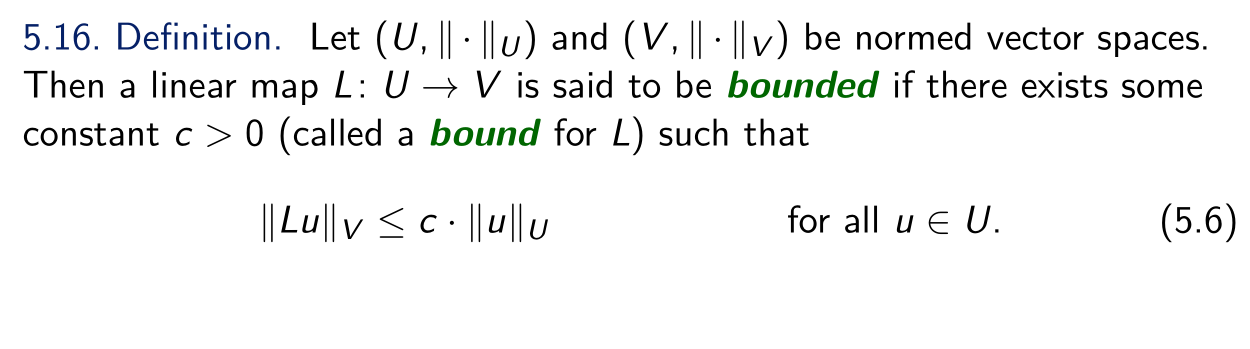
\includegraphics[width=\textwidth]{2020-05-25-17-16-51.png}
    \end{figure}

    \remark  It can be shown that if $U$ is a finite-dimensional vector space, then any linear map is bounded. (You will prove this in VV286, following from the fact that \textbf{any two norms on a finite-dimensional space are equivalent}.)
\end{frame}

\begin{frame}
    \frametitle{Operator Norm}
    \begin{figure}[H]
        \centering
        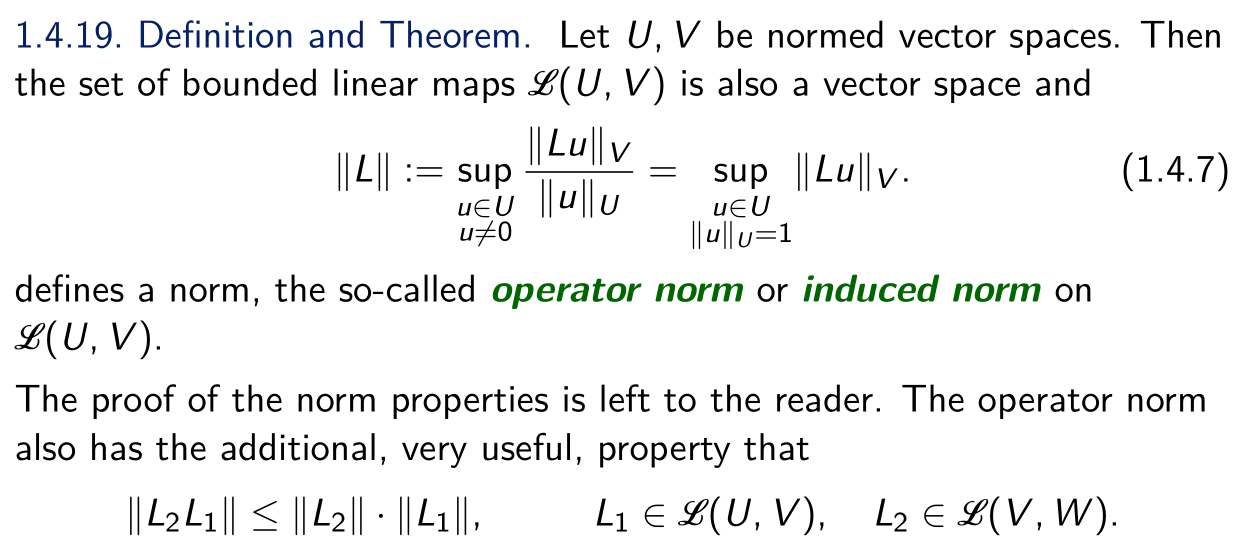
\includegraphics[width=\textwidth]{2020-05-25-17-34-13.png}
    \end{figure}

    \remark Operator norm is quite useful due to its good property. Try to prove this property.
\end{frame}

\section{Matrices}
\begin{frame}
    \frametitle{Overview}
    \begin{enumerate}
        \item Definition of Matrix
        \item \textbf{Matrices as Linear Maps}
        \item Matrix Product
        \item Matrix Transpose/Adjoint
        \item Property of Matrices
        \item Matrix Inverse
        \item Change of Basis
    \end{enumerate}
\end{frame}

\subsection{Definition of Matrix}
\begin{frame}
    \frametitle{Definition of Matrix}
    Since that
    \begin{itemize}
        \item Every n-dimensional real vector space is isomorphic to $\R^n$;
        \item Every n-dimensional complex vector space is isomorphic to $\C^n\cong  \R^{2n}$;
    \end{itemize}
    we only need to focus on $\mathcal{L}(\R^n,\R^m)\cong \text{Mat}(m\times n;\F)$.\\
    An $m\times n$ matrix over the matrix over the complex numbers is a map
    \[a:\{1,\ldots,m\}\times\{1,\ldots,n\}\to\C,\qquad\qquad(i,j)\mapsto a_{ij}.\]
    We represent the graph of $a$ through
    \begin{equation*}
        A:=\begin{pmatrix}
            a_{11} & a_{12} & \cdots & a_{1n} \\
            a_{21} & a_{22} & \cdots & a_{2n} \\
            \vdots & \vdots & \ddots & \vdots \\
            a_{m1} & a_{m2} & \cdots & a_{mn}
        \end{pmatrix}=(a_{ij})_{\begin{subarray}~1\leq i\leq m\\ 1\leq j\leq n\end{subarray}}.
    \end{equation*}
\end{frame}

\subsection{Matrices as Linear Maps}
\begin{frame}
    \frametitle{\textbf{Matrices = Linear Maps}}
    We consider matrices and linear maps as \emph{actually identical} because
    \begin{itemize}
        \item every linear map between finite-dimensional vector spaces may be expressed as a matrix, and
        \item every matrix corresponds (in a certain way) to some such linear map.
    \end{itemize}
    Each matrix $A\in\text{Mat}(m\times n;\R)$ uniquely determines a linear map $j(A)\in\mathcal{L}(\R^n,\R^m)$ such that \textbf{the columns $a_{\cdot k}$ are the images of the standard basis vectors $e_k\in\R^n$}; in particular,
    \[j:\text{Mat}(m\times n;\R)\to\mathcal{L}(\R^n,\R^m)\]
    is an isomorphism, Mat$(m\times n;\R)\cong\mathcal{L}(\R^n,\R^m)$, so every map $L\in\mathcal{L}(\R^n,\R^m)$ corresponds to a matrix $j^{-1}(L)$ whose columns $a_{\cdot k}$ are the images of the standard basis vectors $e_k\in\R^n$.
\end{frame}

\begin{frame}
    \frametitle{\textbf{Matrices = Linear Maps}}
    \remark This theorem is extremely important for us to understand the essence of matrices —— \textbf{They are nothing special but just linear maps} defined in certain way. Recall the sentence on the cover page of my slide:

    \begin{quote}
        \center
        ``Matrices are just linear maps!''\\
    \end{quote}
    Another golden rule to keep in mind
    \begin{quote}
        ``The columns of the matrix are the images of the standard basis vector.”
    \end{quote}
\end{frame}

\begin{frame}
    \frametitle{\textbf{Matrices = Linear Maps}}
    Why is this equivalency so important? Because inspired by this theorem we can further define the operation of matrices, prove some cool properties of matrices, and etc. It will greatly help you understand what's going on in the future study of linear algebra.

    For example, we will soon show that the derivatives of a vector function is actually a matrix! Why is that? Recall that the derivative is the linear approximation of the original function at some point. And a matrix is just a linear map! Then it immediately makes sense.

\end{frame}

\begin{frame}
    \frametitle{\textbf{Matrices = Linear Maps}}


\end{frame}

\subsection{Matrix Product}
\begin{frame}
    \frametitle{Matrix Product}
    Let $A\in\text{Mat}(l\times m;\C)$ and $B\in\text{Mat}(m\times n;\C)$. Then the product of $A$ and $B$ is
    $$\begin{pmatrix}
            Ab_1,Ab_2,...,Ab_j
        \end{pmatrix}$$
    The result of matrix multiplication is that we apply $A$ to each column of $B$.
\end{frame}

\subsection{Matrix Transpose/Adjoint}
\begin{frame}
    \frametitle{Matrix Transpose/Adjoint}
    For $A=(a_{ij})\in\text{Mat}(m\times n;\F)$ we define the \emph{transpose} of $A$ by
    \[A^T\in\text{Mat}(n\times m;\F),\qquad\qquad\qquad A^T=(a_{ji}).\]

    We also define the \emph{adjoint}
    \[A^*\in\text{Mat}(n\times m;\F),\qquad\qquad\qquad A^*=\overline{A}^T=(\overline{a_{ji}}).\]
    where in addition to the transpose the complex conjugate of each entry is
    taken.\\[9pt]
    It is easy to see (in the assignments) that for $A\in\text{Mat}(m\times n;\F),~x\in\F^m,~y\in\F^n$,
    \[\scp{x}{Ay}=\scp{A^*x}{y}.\]
\end{frame}

\subsection{Matrix Properties}
\begin{frame}
    \frametitle{Matrix Properties}
    \begin{itemize}
        \item Not commutative for product. $AB\neq BA$
        \item Associative for product. $(AB)C=A(BC)$
        \item commutative for sum. $A+B=B+A$
        \item Associative for sum. $A+B+C=A+(B+C)$
        \item Right and left distributive for product. $A(B+C)=AB+AC$ and $(D+E)F=DF+EF$
        \item Transpose of product. $(AB)^T=B^TA^T$
        \item Transpose of sum. $(A+B)^T=A^T+B^T$
        \item Transpose \& Inverse. $(A^T)^{-1}=(A^{-1})^T$
        \item Inverse of two invertible matrix's product (if exists) $(AB)^{-1}=B^{-1}A^{-1}$
    \end{itemize}
\end{frame}

\begin{frame}
    \frametitle{Matrix Trace}
    For $A=\left(a_{i j}\right)_{i, j=1}^{n} \in \operatorname{Mat}(n \times n, \mathbb{C})$ we define the \emph{trace} $$\operatorname{tr} A:=\sum_{i=1}^{n} a_{i i}$$

    \textbf{Properties}:
    \begin{itemize}
        \item $\operatorname{tr} i d_n=n$
        \item $\operatorname{tr}(A+B)=\operatorname{tr} A+\operatorname{tr} B $
        \item $\operatorname{tr} A^{T}=\operatorname{tr} A    $
        \item $\operatorname{tr}\left(A H^{T}+H A^{T}\right)=2 \operatorname{tr} A H^{T}$ (How to prove?)
    \end{itemize}
    \nullspace
    \textbf{Remark}: Always give your answer in the most concise way (in exams).
\end{frame}

\begin{frame}
    \frametitle{Comments from Former TAs}
    This is the part of an announcement for mid2 grading last year.
    \nullspace
    \begin{quote}
        To start with, most of you finished your solution with $\operatorname{tr}\left(A^{T} H+H^{T} A\right)$ (similar for the second derivative). The answer itself is indeed correct. However, I have deducted 1 point since it is equally important to see that $\operatorname{tr} A=\operatorname{tr} A^{T},$ and simplify the answer to $2 \operatorname{tr}\left(A^{T} H\right) .$ There are also some students who write out the answer element-wise, I have also deducted point to sort of balance the grading. In my defense, it is not only important to know how to differentiate abstract object without exhaustively listing its component elementwise, but also you should be able to see it through that $2 \operatorname{tr}\left(A^{T} H\right)$ is the most precise answer".
    \end{quote}

\end{frame}



\subsection{Matrix Inverse}
\begin{frame}[allowframebreaks]
    \frametitle{Matrix Inverse}
    A matrix $A\in\text{Mat}(n\times n;\R)$ is called \emph{invertible} if there exists some $B\in\text{Mat}(n\times n;\R)$ such that
    \begin{equation}\label{eq19}
        AB=BA=\text{id}=\begin{pmatrix}
            1 &        & 0 \\
              & \ddots &   \\
            0 &        & 1
        \end{pmatrix}.
    \end{equation}
    We then write $B=A^{-1}$ and say that $A^{-1}$ is the \emph{inverse} of $A$.\\
    \nullspace\textbf{Exercise}:
    Calculate the inverse of
    \[
        A=\frac{1}{5 \sqrt{2}}\left(\begin{array}{ccc}
                3 & -3 & 2 \sqrt{2}  \\
                4 & -4 & -3 \sqrt{2} \\
                5 & 5  & 0
            \end{array}\right)
    \]
    \newpage
    How to find the inverse of a given matrix?
    \begin{itemize}
        \item Use the Gau\ss-Jordan Algorithm (i.e. to find a series of elementary matrix manipulations to transform the matrix into a unit matrix)
        \item (\textit{8.25. Theorem}) Let $A=(a_{ij})\in\text{Mat}(n\times n)$ be invertible. Then
              \[A^{-1}=\frac{1}{\det A}A^{\sharp}\]
              You will learn this soon.
    \end{itemize}
    \remark
    \begin{itemize}
        \item The inverse is unique. (How to prove?)
        \item We only need to verify $AB=id$ or $BA=id$ to conclude $B=A^{-1}$ by \textit{6.12. Remark.}
        \item However, it is not always true (For finite-dimensional vector space, it is true) that $L_1\circ L_2=id\Rightarrow L_2\circ L_1=id$ for two general linear maps $L_1,L_2$!
    \end{itemize}
\end{frame}

\begin{frame}
    \frametitle{Left Inverse \& Right Inverse}
    Let $l^2$ be space of square summable sequence and $L,R$ be left and right shift defined by
    $$
        \begin{aligned}
             & L:l^2\rightarrow l^2, (a_n)\mapsto(l_n)=(a_{n+1})                  \\
             & R:l^2\rightarrow l^2, (a_n)\mapsto(r_n)=\begin{cases}
                0       & n=0     \\
                a_{n-1} & n\neq 0
            \end{cases}
        \end{aligned}
    $$
    We notice that $L\circ R=id\neq R\circ L$. Hence we say that for $L$, only \textit{right inverse} exists; for $R$, only \textit{left inverse} exists.\nullspace
    \textbf{Question}: What is the adjoint of $L,R$? (Hint: use the definition of adjoint in your assignment.)
\end{frame}

\begin{frame}
    \frametitle{Left Inverse \& Right Inverse}
    \pause $L^*=R\quad R^*=L$
\end{frame}

\begin{frame}
    \frametitle{Exercise}
    Let $N$ be a square matrix. We say that $N$ is \emph{nilpotent} if there exists a positive integer $r$ such that $N^{r}=0 .$ where $0$ is the zero matrix. Prove that if $N$ is nilpotent then $N-$id is invertible

    (Hint: id$^r-N^r=$ id)

\end{frame}

\subsection{Change of Basis}
\begin{frame}
    \frametitle{Change of Basis}
    \small Change of basis, especially from the passive view, is sometimes hard to understand. What are we doing when we add some linear transform $T$ to the vector $x$? \textbf{We are essentially apply $T^{-1}$ to the given basis of that space.} The coordinate system is not an inherent part of the space. For example, a physical law should hold no matter what coordinate systems we choose. It is like we merely describe the same thing in different languages! Inspired by this, we might prefer to use the passive view.\\
    In brief,
    \begin{itemize}
        \item In an active transformation, given a basis, we start from a vector and we find a new vector in the same basis.
        \item In a passive transformation we have a vector expressed in a basis and we express it in a new basis.
    \end{itemize}
    \textbf{Extension}:
    \href{https://www.youtube.com/watch?v=P2LTAUO1TdA}{Change of Basis - 3B1B}
\end{frame}

\begin{frame}
    \frametitle{Example}
    Why do we want to change the basis?\\[9pt]
    \pause
    One possible situation is, we can decrease the computing complexity in certain coordinate systems. You will learn \emph{tensor of inertia} in \textit{VP160}. It is a $3\times 3$ self-adjoint matrix that describe how distribution of an object's mass affects its rotation. Specifically,
    $$L=I\omega$$
    where $L\in \R^3$ is angular momentum, $I\in \text{mat}(3\times 3;\R)$ is the tensor of inertia, and $\omega\in\R^3$ is angular velocity.
    If we can rotate the coordinate system, so that $I$ is in a diagonal form:
    $$
        I=\begin{pmatrix}
            \lambda_1 & 0         & 0         \\
            0         & \lambda_2 & 0         \\
            0         & 0         & \lambda_3
        \end{pmatrix}
    $$
    we can dramatically simplify the computation.
\end{frame}

\begin{frame}
    \frametitle{Remarks about Assignment 2}
    You should attach importance to these new concepts in the assignment:
    \begin{itemize}
        \item Dual space
        \item Matrix elements
        \item \textbf{Adjoint}
        \item Orthogonal matrix
        \item \textbf{Range-Kernel decomposition}
        \item Projection
        \item \textbf{Trace}
    \end{itemize}
\end{frame}

\begin{frame}
    \frametitle{Discussion}
    \vspace{1cm}
    \begin{center}
        \LARGE
        Have Fun\\
        And\\
        Learn Well!
    \end{center}


\end{frame}

\end{document}